\section{The Orienteering Problem} % (fold)
\label{sec:02:problem}

This formulation is inspired by \citeauthor{vansteenwegen_orienteering_2011} \cite{vansteenwegen_orienteering_2011}.
Let $G=(V,E)$ be an undirected graph with a set of vertices $V = \{v_1, \dots, v_n\}$ and a set of edges $E$.
In addition let $t: E \rightarrow \mathbb{R}_+$ be a function assigning a travel time to each edge of the graph and let
$s: V \rightarrow \mathbb{R}_+$ be a function assigning a score to each vertex.
For $v_i, v_j \in V$ we write $t(v_i, v_j) := t(\{v_i, v_j\})$ for simplicity.
Also let $T_{max} \in \mathbb{R}_+$ be a time limit.

The objective of the \emph{Orienteering Problem} is to find a path starting at $v_1$ and ending at $v_n$ 
such that the sum of its score is maximized while still respecting the time bound $T_{max}$.
More formally, find $P = (p_1, \dots, p_k)$, $p_i \in V,\ i=1,\dots, k$ for some $1 \leq k \leq n$ where $p_1 = v_1$ and $p_k = v_n$ such that

\begin{align*}
  \sum_{i = 2}^k t(p_{i-1}, p_i) \leq T_{max}
\end{align*}

holds and

\begin{align*}
  \sum_{v_i \in P} s(i)
\end{align*}

is maximized.

\unsure{Maybe talk about the ILP representation of the OP}

While the above definition forms the base of the OP, the solutions found in the literature restrict the types of graphs that are allowed as input.
We will introduce some restrictions prevalent in the literature in ascending order of their strictness. 

\subsection{Completeness}
\label{subsec:02:complete}

A graph is \emph{complete} if and only if for any two nodes $v_i \neq v_j \in V$, there exists a corresponding edge $\{v_i, v_j\} \in E$.
An almost unanimous \cite{vansteenwegen_orienteering_2011} restriction in the literature regarding the OP and its variants is the requirement of graph completeness. \cite{szwarc_novel_2022,vansteenwegen_orienteering_2011,laporte_selective_1990,santini_hazardous_2022}

This allows simplifying algorithms while not being too restrictive.
One could insert missing edges into an incomplete graph by for example choosing the time of the shortest path in the preexisting graph for each missing edge's weight.
However, this of course would require additional computation which might be expensive on large inputs.

If it is not desired for the missing edges to be traversable,
edges with a weight of $\infty$ or a weight greater than $T_{max}$ could be chosen.
Note, that this method may not work for all algorithms. Examples of this will be discussed later. (see \cref{subsec:03:salgo})

\subsection{Triangle Inequality}
\label{subsec:02:triangle}

According to the NIST Dictionary of Algorithms and Data Structures \cite{black_triangle_2004} a complete,
weighted graph satisfies the \emph{triangle inequality} if the following condition holds:
Any three vertices $u \neq v \neq w \in V$ satisfy the inequation
\begin{align*}
  t(u, w) \leq t(u, v) + t(v, w) 
\end{align*}
where again the function $t$ represents the weight of the edge between the given nodes.

Since this definition requires the graph to be complete and therefore entails the requirement described in \cref{subsec:02:complete}.
Intuitively this means that there is no path between nodes $u$ and $w$ that has a strictly lesser weight
than the direct edge $\{u, w\}$. So no \enquote{detour} will ever be faster than the direct path. 

This requirement is less frequently explicitly stated \cite{santini_hazardous_2022} but more often implied by requiring a Euclidean metric (see \cref{subsec:02:euclidean}).

The benefit of operating on a graph that satisfies the triangle inequality
is that it provides a significant advantage to algorithms that take advantage of it.
(see \cref{subsec:03:salgo}) \todo{cite HS here if included}

\begin{figure}
  \centering
  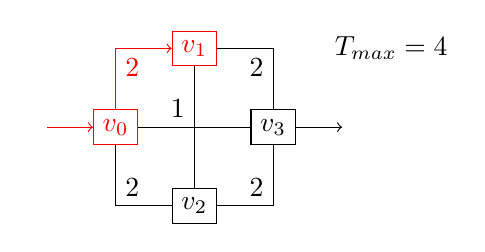
\begin{tikzpicture}[vertex/.style={draw, shape=rectangle}]
    \node at (3.5, 1) {$T_{max}=4$};
    \node at (-1,0) (invis) {};
    \node[vertex, red] at (0, 0) (0) {$v_0$};
    \node[vertex, red] at (1, 1) (1) {$v_1$};
    \node[vertex] at (1,-1) (2) {$v_2$};
    \node[vertex] at (2, 0) (3) {$v_3$};
    \node at (3,0) (invis2) {};

    \draw[->, red] (invis) -- (0);
    \draw[->, red] (0) |- node[below right] {$2$} (1);
    \draw (0) |- node[above right] {$2$} (2);
    \draw (1) -- node[above left] {$1$} (2);
    \draw (0) -- (3);
    \draw (1) -| node[below left] {$2$} (3);
    \draw (2) -| node[above left] {$2$} (3);
    \draw[->] (3) -- (invis2);
  \end{tikzpicture}
  \caption{A complete graph that satisfies the triangle inequality. 
  The start node is marked by an inward-facing arrow and the end node by an outward-facing arrow. 
  The edges and nodes marked in red are the edges the algorithm has so far included in its solution to the OP.}
  \label{fig:02:example_triangle}
\end{figure}

An example is depicted in \cref{fig:02:example_triangle}. The algorithm began its search at the starting node $v_0$ and made its way to node $v_1$.
Now the cost of the path is already $2$. $T_{max}$ being $4$, the path only has remaining capacity of $2$ left.
The algorithm now has the choice between moving to $v_2$ or the end node $v_3$. As the weight of the edge $\{v_1, v_3\}$ is $2$, we could complete the path while respecting our budget $T_{max}$.
However, we might want to know whether a route including $v_2$ would be more profitable while also respecting our budget.

In our case, we see that if we were to travel to $v_2$ our remaining capacity would be $1$.
If we then tried to travel to $v_3$ (edge weight $2$) it would violate the constraint.
Knowing that the graph satisfies the triangle equality, we now know that we cannot include $v_2$ in our path, since the edge $\{v_2, v_3\}$ is the shortest path between these two nodes and even this one violates our budget.
Therefore, there can be no other path including $v_2$ that respects our budget. 
So we can skip this node without any further exploration of all paths that would include $v_2$. 

Were the graph not to fulfill the triangle inequality, then there would be no simple way to tell whether a path involving $v_2$ could respect our budget.
After all, there could be another path between $v_2$ and $v_3$ with a weight of at most $1$.

As we can see, the triangle inequality allows algorithms to use a simple method to determine whether a node can be added to a path.

\subsection{Euclidean Metric}
\label{subsec:02:euclidean}

The strictest prevalent restriction is the assumption of a Euclidean metric. 
That is, each node $v_i \in V$ has coordinates $(x_i, y_i)^\intercal \in \mathbb{R}^2$ associated with it.
In addition: 
\begin{align*}
  t(v_i,v_j) := \sqrt{(x_i - x_j)^2 + (y_i - y_j)^2},\ \forall i \neq j
\end{align*}

So the weight of each edge is the Euclidean distance between them. Note, that this also implies that the graph is complete.
Since the Euclidean distance is a metric, it also satisfies the triangle inequality.
It follows that this metric entails the restrictions from \cref{subsec:02:complete,subsec:02:triangle}.

As stated by \citeauthor{vansteenwegen_orienteering_2011} in their survey paper on this topic \cite{vansteenwegen_orienteering_2011}, the OP's definition is general, however the algorithms described in the literature in general are in respect to such Euclidean graphs. \cite{golden_orienteering_1987,tsiligiridis_heuristic_1984,szwarc_novel_2022,geem_harmony_2005}.

However, some approaches might even work as is on graphs with only the previous two restrictions (see \cref{subsec:03:salgo}) or they may be adapted to work with such graphs while perhaps losing some of their quality. %(see \cref{sec:04:szwarc}). 

\subsection{Possible Reasons}
\label{subsec:02:reasons}

If one looks at examples of applications of the Orienteering Problem and its variants to real-world routing problems,
some reasons for these restrictions might become apparent. Examples are:
\begin{itemize}
  \item The scenario mentioned in \cref{sec:01:introduction} in which a salesman searches for a route between cities while maximizing his profit. \cite{chao_fast_1996}
  \item A logistic company planning routes for a vehicle collecting hazardous but profitable parcels from clients while minimizing the time they are in transit for fear of them leading to all profit being lost. \cite{santini_hazardous_2022}    
  \item Planning tours through a country while trying to maximize the enjoyment of the tour while having a restriction on the maximum travel distance. \cite{geem_harmony_2005}
  \item The original sport of orienteering which inspired the name of the OP. \cite{tsiligiridis_heuristic_1984}  
\end{itemize}

As they relate to the real world, modeling them in terms of the OP or variants thereof 
will result in an input akin to ones described in \cref*{subsec:02:euclidean}, 
with the nodes having a location in space and the distance between them being at least roughly proportional to the Euclidean distance between them.

As such, if one wanted to solve these problems assuming the input to be Euclidean is likely to be a fairly accurate approximation of the real-world problem one is trying to solve and in addition provides more knowledge to work with when trying to design an algorithm.
If one perused the test instances compiled by \citeauthor{vansteenwegen_orienteering_2011} \cite{vansteenwegen_orienteering_2011}, 
one would find, that these are all Euclidean. 

So while these restrictions might not be that helpful when trying to solve the general OP, it is also unsurprising that this focus exists in the literature.
However, this is not to say that this is the primary let alone the only reason why this is the case.

We will now introduce algorithms from the literature and discuss 
whether the requirements and heuristics originally described in the paper can be relaxed without sacrificing too much of the algorithm's functionality.
To explore this, we will take a look at algorithms by \citeauthor{tsiligiridis_heuristic_1984}. \cite{tsiligiridis_heuristic_1984}
%older \cite{tsiligiridis_heuristic_1984} and one recent \cite{szwarc_novel_2022} solution approach to the orienteering problem.
% section 02:problem (end)